\documentclass[11pt]{article}

\usepackage{fancyhdr} 
\usepackage{lastpage}
\usepackage{extramarks} 
\usepackage{graphicx} 
\usepackage{enumitem}
\usepackage{mcode}
\usepackage{graphicx}
\usepackage{hyperref}
\usepackage{float}
\usepackage[parfill]{parskip}
\usepackage{amsmath}

% Margins
\topmargin=-0.45in
\evensidemargin=0in
\oddsidemargin=0in
\textwidth=6.5in
\textheight=9.0in
\headsep=0.25in 

\linespread{1} % Line spacing

% Custom macros

% Set up the header and footer
\pagestyle{fancy}
\lhead{\hmwkClass: \hmwkTitle} % Top left header
\chead{} % Top center header
\rhead{\hmwkAuthorName \firstxmark} % Top right header
\lfoot{\lastxmark} % Bottom left footer
\cfoot{} % Bottom center footer
\renewcommand\headrulewidth{0.4pt} % Size of the header rule

\setlength\parindent{0pt} % Removes all indentation from paragraphs
   
%----------------------------------------------------------------------------------------
%	NAME AND CLASS SECTION
%----------------------------------------------------------------------------------------

\newcommand{\hmwkTitle}{Lab 3} % Assignment title
\newcommand{\hmwkDueDate}{12/8/2016} % Due date
\newcommand{\hmwkClass}{ENEE 222} % Course/class
\newcommand{\hmwkAuthorName}{Anton Lagergren and Erik Holum} % Your name

%----------------------------------------------------------------------------------------
%	TITLE PAGE
%----------------------------------------------------------------------------------------

\title{
\vspace{2in}
\textmd{\textbf{\hmwkClass:\ \hmwkTitle}}\\
\normalsize\vspace{0.1in}\small{Due\ on\ \hmwkDueDate}\\
\vspace{0.1in}\large{\textit{\hmwkClassInstructor\ \hmwkClassTime}}
\vspace{3in}
}

\author{\textbf{\hmwkAuthorName}}
\date{} % Insert date here if you want it to appear below your name

%----------------------------------------------------------------------------------------

\begin{document}

% \maketitle


\section{Abstract}

On an high level, the purpose of this lab is to understand how to analyze, manipulate, and understand frequencies of audio recordings. In the first sections, we examine the notions of voiced, unvoiced, and silenced speech, and how we can identify them using energy levels and a zero-crossing rate. In sections 5, 6, and 7, we work to understand the frequency spectrum of the preceding speech types, and try to implement a function to differentiate them using only frequency analysis. In the final sections, we examine noise filtering through built in Matlab functions, and how we can remove added gaussian white noise from our recordings to recover the original signal.

\section{Body}
In this section we provide the code and methods used for each of the parts defined in the lab manual. We include the results, plots, etc in the results section, as well as any other code used. Specific functions used can be found in the Code section of this report.

\subsection{Parts 1, 2, 3, 4}
% 
% Part 1
%
We begin by record the phrase 'I love Matlab', and saving the speech as a '.wav' file. Note this process is repeated for any other sound recording file used.
\begin{lstlisting} 
% Part 1 record sounds
fs = 10000;
r = audiorecorder(fs,16,1); % Record at fs = 10000
recordblocking(r, 8);
audiowrite('holum.wav', r.getaudiodata, fs); % Save data as .wav

% Part 2, read in sound data
[sp, fs] = audioread('holum.wav');
plot(sp);
\end{lstlisting}

We used the templates provided online as a template for constructing a method of determining voiced, unvoiced, and silenced portions of a recording that used both energy levels and zero-crossings. In particular, we defined a function that took a recording, sample rate, zero-crossing threshold, energy threshold, and a silence energy threshold, that separated the given vector in three equally sized vectors containing the results. See the code section for implementations of the functions used in the following script. In particular, 

The method is documented in: 

https://www.asee.org/documents/zones/zone1/2008/student/ASEE12008\_0044\_paper.pdf

\begin{lstlisting}
zc_threshold = 0.100; % zero_crossings / num_samples
en_threshold = 0.075; % Energy threshold
silence_en_threshold = 0.03; % Silence energy threshold
fsize = 1000;

%
% Identify voiced, unvoiced, and silence from basic recording
%
sound_file = 'holum.wav';
[speech, fs] = audioread(sound_file);

[voiced, unvoiced, silence, t] = part_3(speech, fs, zc_threshold, ...
    en_threshold, silence_en_threshold, fsize);

hold off;
subplot(4,1,1);
plot(t, speech);
title('Plot of Standard Recording');
ylabel('Amp');
xlabel('time (s)');

subplot(4,1,2);
plot(t, voiced, 'b');
hold on;
plot(t, unvoiced, 'r');
plot(t, silence, 'g');
legend('voiced', 'unvoiced', 'silence')
title('Plot of Voiced/Unvoiced/Silence for Standard Recording');
ylabel('Amp');
xlabel('time (s)');
hold on;
\end{lstlisting}

% 
% Part 4
%
We then went on and used the provided files to add gaussian white noise to our recording, and repeated the process using the part\_3.m Matlab script.

\begin{lstlisting}
%
% Try 5db of noise to recording and repeat part 3.
%
sound_file = 'noisy_speech.wav';
[nsp, fs] = audioread(sound_file);

[voiced, unvoiced, silence, t] = part_3(nsp, fs, zc_threshold, ...
    en_threshold, silence_en_threshold, fsize);

subplot(4,1,3);
plot(t, nsp);
title('Plot of Noisy Recording');
ylabel('Amp');
xlabel('time (s)');

subplot(4,1,4);
plot(t, voiced, 'b');
hold on;
plot(t, unvoiced, 'r');
plot(t, silence, 'g');
legend('voiced', 'unvoiced', 'silence')
title('Plot of Voiced/Unvoiced/Silence for Noisy Recording');
ylabel('Amp');
xlabel('time (s)');
\end{lstlisting}


\subsection{Parts 5, 6, 7}

For part 5, we used the labeled waveforms from from part 3 to find specific time indexes that we knew to be unvoiced, voiced, or silenced. Then produced plots of the ffts of those segments to get an idea of the spectrum of each kind of speech. We used the following to manually locate unvoiced segments, and plot them together. Note we grabbed segments from two separate unvoiced locations, i.e. different words.

\begin{lstlisting}
clc;
clear;
close all;
clear plot;

sound_file = 'noisy_speech.wav';
[nsp, fs] = audioread(sound_file);

sound_file = 'holum.wav';
[speech, fs1] = audioread(sound_file);

% Unvoiced segments determined in the previous section
seg1 = nsp(31001:31500);
seg2 = nsp(31501:32000);
seg3 = nsp(32001:32500);

seg4 = nsp(48001:48500);
seg5 = nsp(48501:49000);
seg6 = nsp(49001:49500);

N = 1024;

% display ffts for unvoiced segments (only doing 3, they all look basically
% the same.
subplot(2,1,1)
for s=[seg1 seg2 seg3]
    X = abs(fft(s,N));
    X = fftshift(X);
    F = [-N/2:N/2-1]/N;
    plot(F,X);
    hold on
end
xlabel('frequency / f s');
legend('seg1', 'seg2', 'seg3');
grid
title('ffts for first segment');

subplot(2,1,2)
for s=[seg4 seg5 seg6]
    X = abs(fft(s,N));
    X = fftshift(X);
    F = [-N/2:N/2-1]/N;
    plot(F,X);
    hold on
end
xlabel('frequency / f s');
legend('seg4', 'seg5', 'seg6');
grid
title('ffts for second segment');

pause
\end{lstlisting}

We also used the fft function to compare voiced, unvoiced, and silence fits.
\begin{lstlisting}
% Plot comparisons of voiced, unvoiced, and silence ffts
hold off;
seg = nsp(46001:46500);
X = abs(fft(seg,N));
X = fftshift(X);
F = [-N/2:N/2-1]/N;
plot(F,X);
hold on

X = abs(fft(seg1,N));
X = fftshift(X);
F = [-N/2:N/2-1]/N;
plot(F,X);
hold on
    
seg = nsp(25001:25500);
X = abs(fft(seg,N));
X = fftshift(X);
F = [-N/2:N/2-1]/N;
plot(F,X);

grid;
title('Comparison of Voiced, Unvoiced, and Noise ffts');
legend('voiced', 'unvoiced', 'noise');

pause;
\end{lstlisting}

Finally, we used the script in part\_7.m to repeat part 3, this time using the fft to determine whether or not a segment is voiced, unvoiced, or silent. The code for the function is available in the Code section, and additional discussion about different methods tried is in the results and discussion section.

\begin{lstlisting}
% Based on the above information, do something with part 7 to identify
% voiced/etc
voiced_model = nsp(46001:46500);
unvoiced_model = nsp(31001:31500);

% regular
[voiced, unvoiced, silence, t] = part_7(speech, fs, N, 500, ...
    voiced_model, unvoiced_model, .4);
subplot(2,1,1);
plot(t, voiced, 'b');
hold on;
plot(t, unvoiced, 'r');
plot(t, silence, 'g');
legend('voiced', 'unvoiced', 'silence')
title('Identification using FFT on Standard Recording');
ylabel('Amp');
xlabel('time (s)');
grid;
hold on;

% noisy
[voiced, unvoiced, silence, t] = part_7(nsp, fs, N, 500, ...
    voiced_model, unvoiced_model, .4);
subplot(2,1,2);
plot(t, voiced, 'b');
hold on;
plot(t, unvoiced, 'r');
plot(t, silence, 'g');
legend('voiced', 'unvoiced', 'silence')
title('Identification using FFT on Standard Recording');
ylabel('Amp');
xlabel('time (s)');
grid;
hold on;
\end{lstlisting}


\subsection{Parts 8,9}
Finally, we experimented with different kinds of filtering to remove noise (or increase the signal to noise ratio?) of our recordings. We started with a simple moving average filter, then experimented with other filter functions in the Matlab library. Including a lowpass, bandpass, and polynomial Savitzky-Golay filter.

\begin{lstlisting}
clc;
clear;
close all;
clear plot;

sound_file = 'noisy_speech.wav';
[nsp, fs] = audioread(sound_file);

N = length(nsp);
x = 1:length(nsp);
t = x./fs;

% Moving average filter
order = 10;
df = (1/order)*ones(1,order);
A = 1;
y1 = filter(df, A, nsp);

% Basic low pass filter fir
df = designfilt('lowpassfir','DesignMethod', ...
      'window','FilterOrder',10,'CutoffFrequency', .05);
y2 = filter(df, nsp); % Apply filter to speech
B = df.Coefficients;

% Passband filter centered around speech 
[df, A] = fir1(10,[0.001 .1]);
y3 = filter(df, A, nsp); % Apply filter to speech

% Savitzky-Golay filtering
y4 = sgolayfilt(nsp, 3, 11);

% Make plots of filtered signals
subplot(5,1,1);
plot(t, nsp);
title('Original Noisy Recording');
grid;
xlabel('time (s)');
ylabel('Amp');

subplot(5,1,2);
plot(t,y1);
title('Moving Average Filter');
grid;
xlabel('time (s)');
ylabel('Amp');

subplot(5,1,3);
plot(t,y2);
title('Basic Low Pass FIR');
grid;
xlabel('time (s)');
ylabel('Amp');

subplot(5,1,4);
plot(t,y3);
title('Basic Band Pass FIR');
grid;
xlabel('time (s)');
ylabel('Amp');

subplot(5,1,5);
plot(t,y4);
title('Savitzky-Golay');
grid;
xlabel('time (s)');
ylabel('Amp');

pause
\end{lstlisting}

For part 9, we again used our script from part 3 to try to separate voiced, unvoiced, and silenced speech from our filtered signals.
\begin{lstlisting}
% Part 9

zc_threshold = 0.100; % zero_crossings / num_samples
en_threshold = 0.075; % Energy threshold
silence_en_threshold = 0.05; % Silence energy threshold
fsize = 500;

[voiced, unvoiced, silence, t] = part_3(nsp, fs, zc_threshold,  ...
    en_threshold, silence_en_threshold, fsize);

subplot(5,1,1);plot(t, voiced, 'b');
hold on;
plot(t, unvoiced, 'r');
plot(t, silence, 'g');
title('Voiced/Unvoiced/Silence Identification');
xlabel('time (s)');
ylabel('Amp');


[voiced, unvoiced, silence, t] = part_3(y1, fs, zc_threshold,  ...
    en_threshold, silence_en_threshold, fsize);

subplot(5,1,2);plot(t, voiced, 'b');
hold on;
plot(t, unvoiced, 'r');
plot(t, silence, 'g');
xlabel('time (s)');
ylabel('Amp');


[voiced, unvoiced, silence, t] = part_3(y2, fs, zc_threshold,  ...
    en_threshold, silence_en_threshold, fsize);

subplot(5,1,3);plot(t, voiced, 'b');
hold on;
plot(t, unvoiced, 'r');
plot(t, silence, 'g');
xlabel('time (s)');
ylabel('Amp');


[voiced, unvoiced, silence, t] = part_3(y3, fs, zc_threshold,  ...
    en_threshold, silence_en_threshold, fsize);

subplot(5,1,4);plot(t, voiced, 'b');
hold on;
plot(t, unvoiced, 'r');
plot(t, silence, 'g');
xlabel('time (s)');
ylabel('Amp');

[voiced, unvoiced, silence, t] = part_3(y4, fs, zc_threshold,  ...
    en_threshold, silence_en_threshold, fsize);

subplot(5,1,5);plot(t, voiced, 'b');
hold on;
plot(t, unvoiced, 'r');
plot(t, silence, 'g');
xlabel('time (s)');
ylabel('Amp');
\end{lstlisting}

%
%
% Results and Discussion Section 
%
%
%
%
\section{Results and Discussion}

\subsection{Parts 1, 2, 3, 4}
As mentioned in the coding section, we used a combination of the zero-crossing method and the energy level method to determine whether or not a segment of our recording was voiced, unvoiced, or silent. 
We should note that we operated under the assumption of what Wikipedia defines as voice vs unvoiced speech (https://en.wikipedia.org/wiki/Voice\_(phonetics)). 
Basically long vowels are unvoiced, hard consonants are voiced, low energy speech is silence. 
Let $E_s$ be the average energy level of a segment, and let $Z_s$ be the percentage of zero-crossings in a segment. 
Then, based on our referenced paper, unvoiced speech should have a high $E_s$ and a high $Z_s$, where as voiced should have high $E_s$ and a low $Z_s$. Silence is taken to be anything below a certain power level, which we call $S_s$. We tuned our levels by recording voiced, unvoiced, and silenced speech, then using our part\_3.m script with different values for $E_s$, $Z_s$, and $S_s$, until we produced plots that were to our liking.

\begin{lstlisting}
% Script in which we determine appropriate levels by analyzing different
% recordings of voiced, unvoiced, and silenced speech.

% https://en.wikipedia.org/wiki/Voice_(phonetics)
fs = 10000;

% Record voiced
%{
r = audiorecorder(fs,16,1); % Record at fs = 10000
recordblocking(r, 4);
audiowrite('voiced.wav', r.getaudiodata, fs); % Save data as .wav
%}


% Record unvoiced
%{
r = audiorecorder(fs,16,1); % Record at fs = 10000
recordblocking(r, 4);
audiowrite('unvoiced.wav', r.getaudiodata, fs); % Save data as .wav
%}


% Record silence
%{
r = audiorecorder(fs,16,1); % Record at fs = 10000
recordblocking(r, 4);
audiowrite('silence.wav', r.getaudiodata, fs); % Save data as .wav
%}

%
% Analyze data and tweak parametersclc;
zc_threshold = 0.135; % zero_crossings / num_samples
en_threshold = 0.075; % Energy threshold
silence_en_threshold = 0.02; % Silence energy threshold
fsize = 500;

% Voiced
sound_file = 'voiced.wav';
[speech, fs] = audioread(sound_file);
[voiced, unvoiced, silence, t] = part_3(speech, fs, zc_threshold, ...
    en_threshold, silence_en_threshold, fsize);
s_voiced = voiced(~isnan(voiced));

% Saved voiced segments
subplot(3,1,1);
plot(t, voiced, 'b');
hold on;
plot(t, unvoiced, 'r');
plot(t, silence, 'g');
legend('voiced', 'unvoiced', 'silence')
title('Plot of Voiced/Unvoiced/Silence for Voiced Recording');
ylabel('Amp');
xlabel('time (s)');
hold on;

% Unvoiced
sound_file = 'unvoiced.wav';
[speech, fs] = audioread(sound_file);
[voiced, unvoiced, silence, t] = part_3(speech, fs, zc_threshold, ...
    en_threshold, silence_en_threshold, fsize);

% Saved unvoiced segments
s_unvoiced = unvoiced(~isnan(unvoiced));
subplot(3,1,2);
plot(t, voiced, 'b');
hold on;
plot(t, unvoiced, 'r');
plot(t, silence, 'g');
title('Plot of Voiced/Unvoiced/Silence for Unvoiced Recording');
ylabel('Amp');
xlabel('time (s)');
hold on;

% Silence
sound_file = 'silence.wav';
[speech, fs] = audioread(sound_file);
[voiced, unvoiced, silence, t] = part_3(speech, fs, zc_threshold, ...
    en_threshold, silence_en_threshold, fsize);

s_silence = silence(~isnan(silence));
subplot(3,1,3);
plot(t, voiced, 'b');
hold on;
plot(t, unvoiced, 'r');
plot(t, silence, 'g');
title('Plot of Voiced/Unvoiced/Silence for Silence Recording');
ylabel('Amp');
xlabel('time (s)');
hold on;

pause;

% Create plots for individual frames
clear plot;
close all;

frame_size = 500;
x = 1:frame_size;
t = x./frame_size;

voiced_frame = s_voiced(1:frame_size);
subplot(3,1,1);
plot(t, voiced_frame);
xlabel('time (s)')
ylabel('Amp')
title('One Frame of Voiced Speech');

unvoiced_frame = s_unvoiced(1:frame_size);
subplot(3,1,2);
plot(t, unvoiced_frame);
xlabel('time (s)')
ylabel('Amp')
title('One Frame of Unvoiced Speech');

silence_frame = s_silence(1:frame_size);
subplot(3,1,3);
plot(t, silence_frame);
xlabel('time (s)')
ylabel('Amp')
title('One Frame of Silenced Speech');
\end{lstlisting}
By varying the thresholds in the preceding script, we were able to get pretty good estimates on what our energy levels and zero-crossing thresholds should be for our normal recording. Based on our evaluation of our recordings, we picked $E_s > 0.075$ to be taken as non-silenced speech, $Z_s > 0.1$ to be unvoiced speech, and $S_s < 0.03$ to be silence. The results are available in figures 1 and 2, including a visualization of voiced vs unvoiced speech, where the difference in $Z_s$ is clearly visible.

\begin{figure}[H]
  \centering
  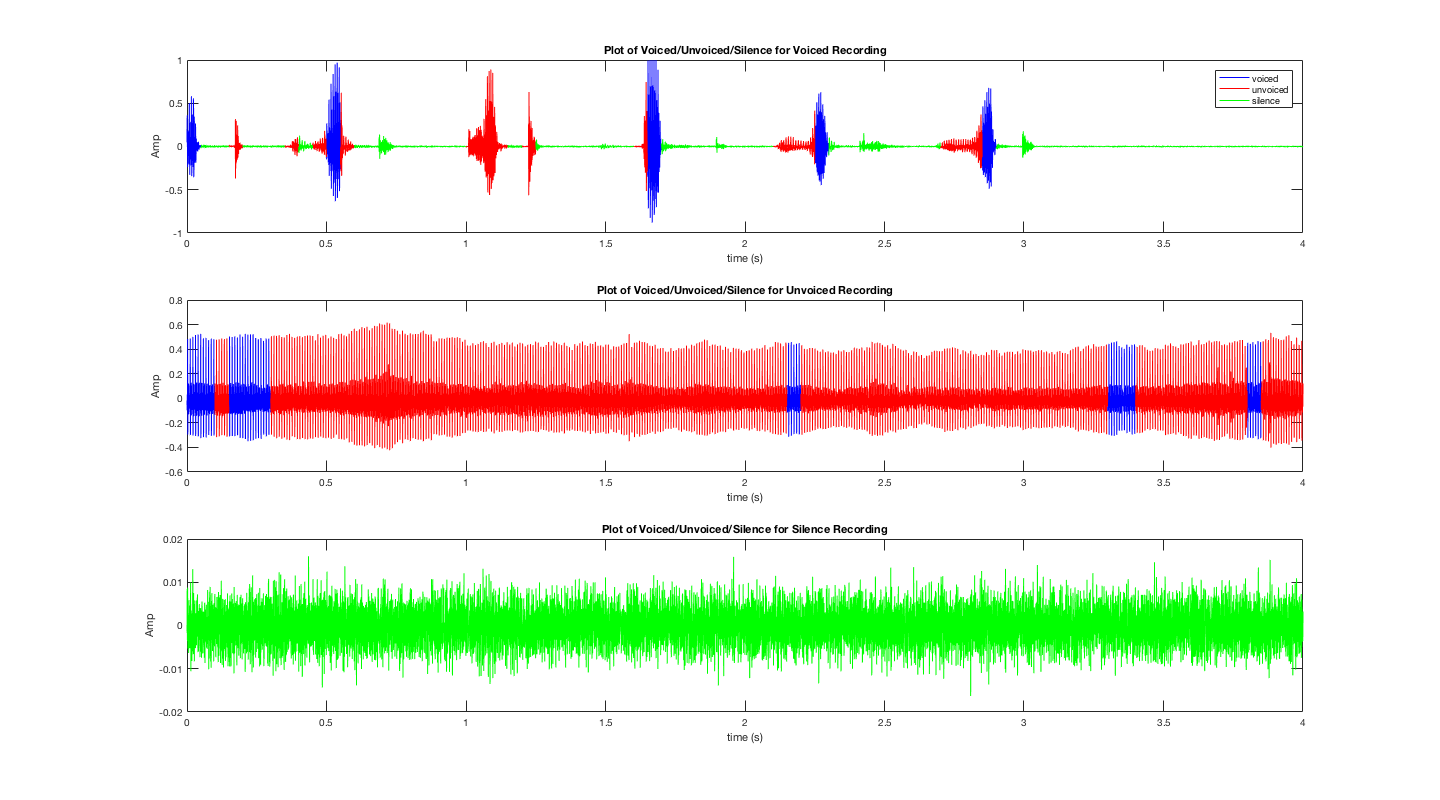
\includegraphics[scale=.25]{speech_tuning_part1.png}
  \caption{Tuning Energy and Zero Crossings}
\end{figure}

\begin{figure}[H]
  \centering
  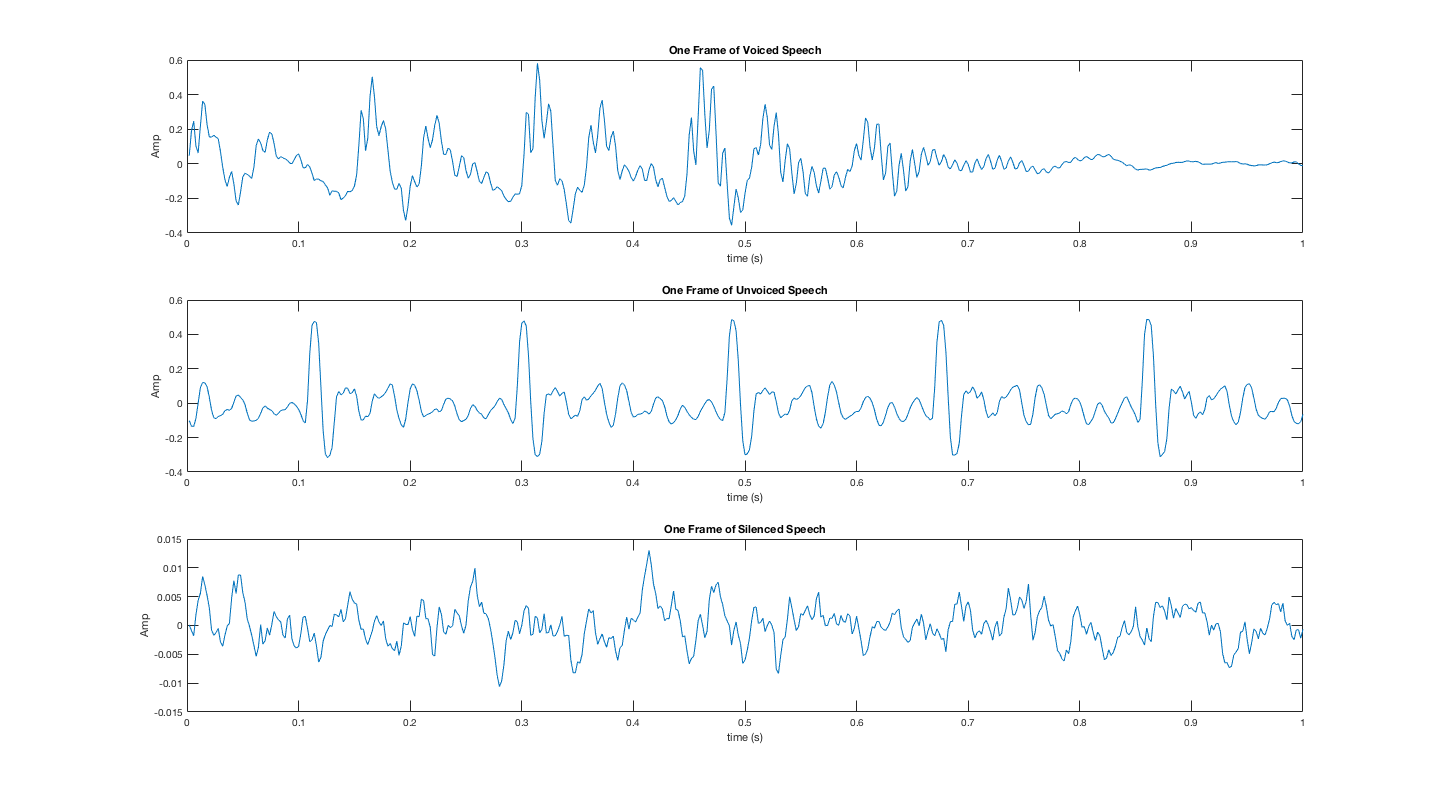
\includegraphics[scale=.25]{speech_tuning_figures.png}
  \caption{Speech Power Levels for Voiced, Unvoiced, and Silence}
\end{figure}

Based on what we discovered in our 'tuning' section, we were able to apply the found values for $E_s$, $Z_s$, and $S_s$ to our both our regular and noisy recordings of 'I love Matlab'. The results are visualized below. We were able to get clear distinctions with no noise, with the hard consonants in 'love' and 'Matlab' clearly coming through. In the noisy recording, however, all of that data was lost, and since the average energy level was universally bumped up by the white noise, all was lost and determined to just be unvoiced speech.

\begin{figure}[H]
  \centering
  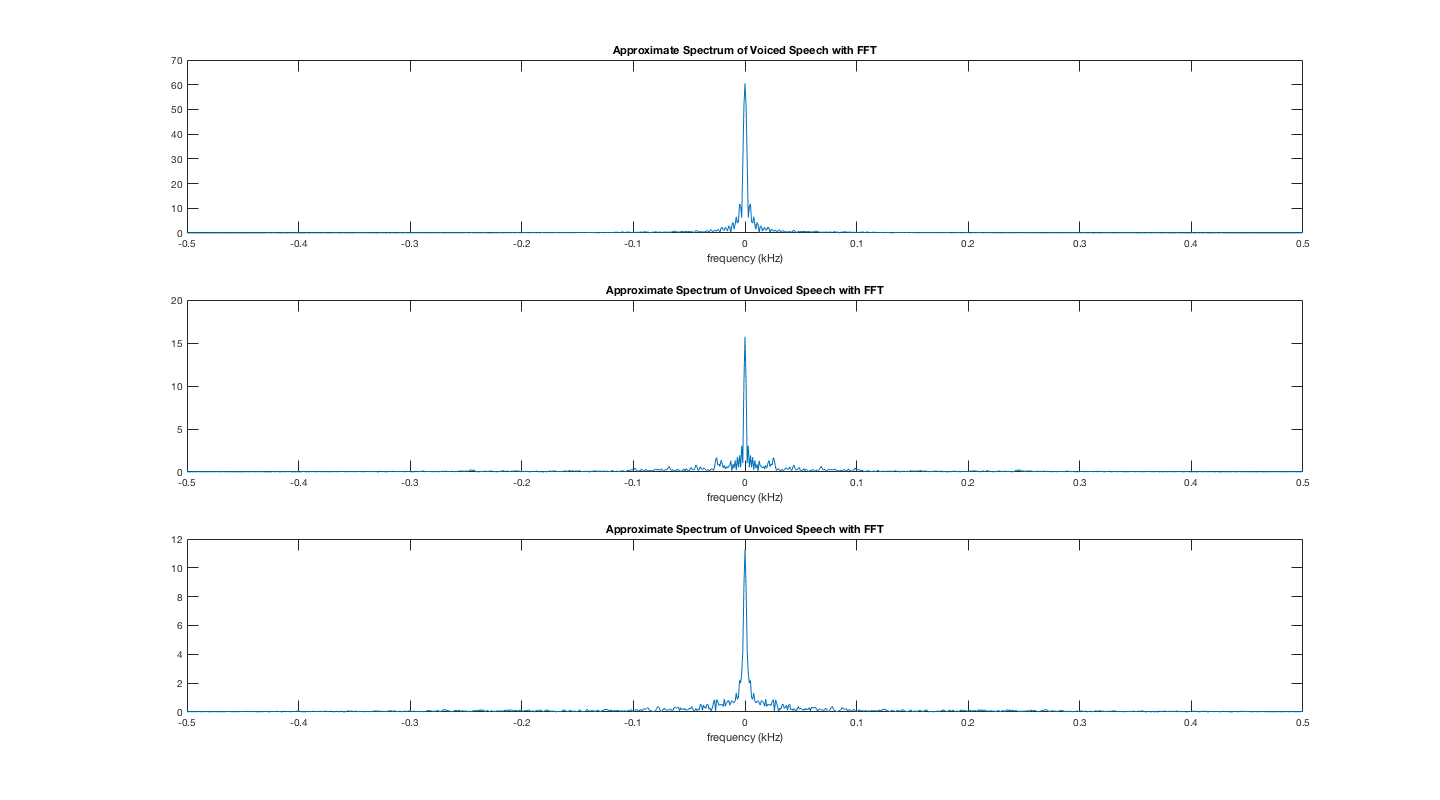
\includegraphics[scale=.25]{part1_spectrums.png}
  \caption{FFTs for Voiced, Unvoiced, and Silence}
\end{figure}

\begin{figure}[H]
  \centering
  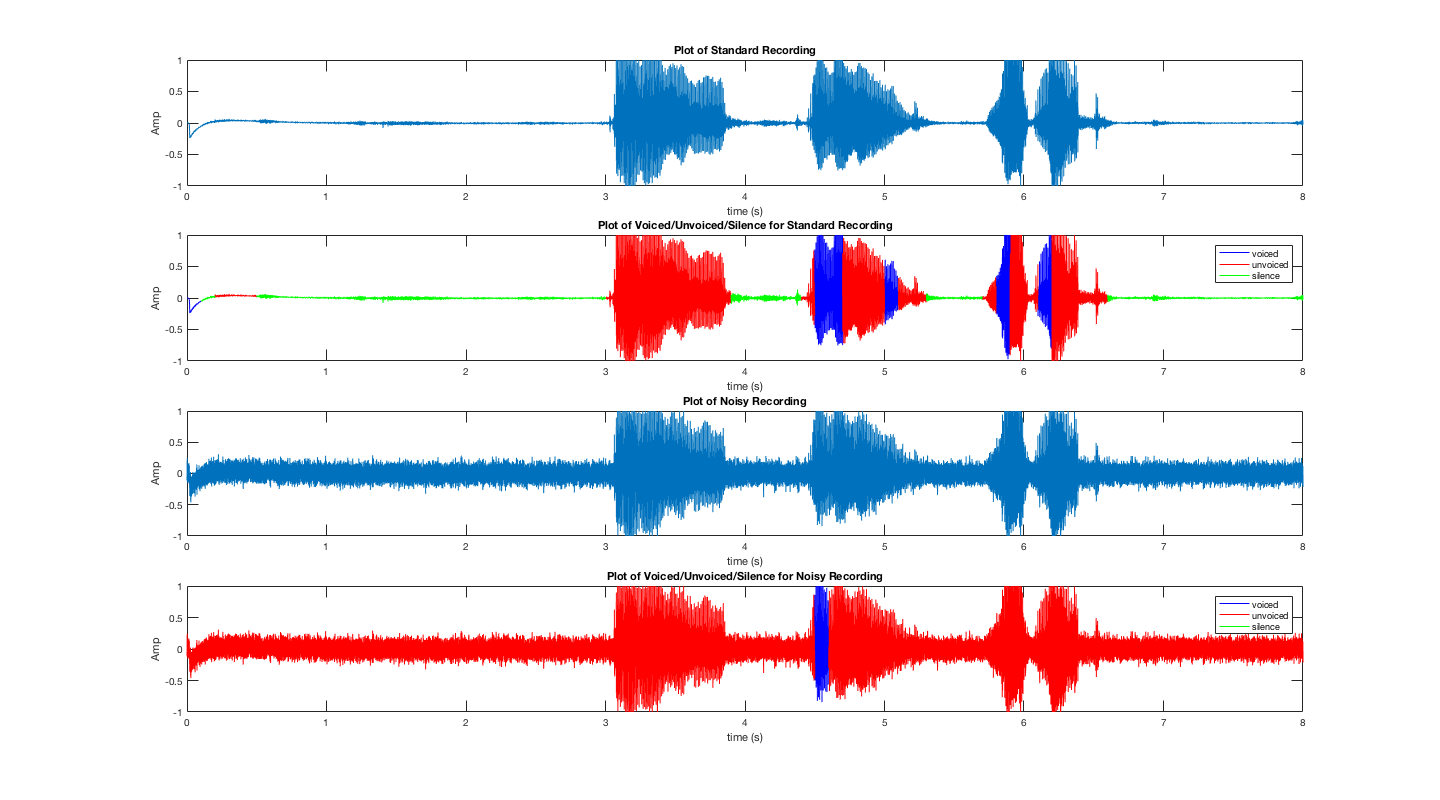
\includegraphics[scale=.25]{part1_4_labeling.png}
  \caption{Labeling Voiced, Unvoiced, and Silence Segments for Regular and Noisy Signals}
\end{figure}


%
%
% Parts 5 6 7
%
%
%
\subsection{Parts 5, 6, 7}
We had some level of success in labeling voiced, unvoiced, and silenced speech using the fft. We began, as noted in the Body section, by manually identifying several unvoiced segments in our noisy recording. We basically chose segments from the 'I' and 'ah' portion of 'Matlab' as our unvoiced samples. The FFTs for three segments of both syllable are visualized in figure 5. To get a better idea of the differences, we also examined ffts from voiced and silenced segments. Those are plotted in figure 6. 

\begin{figure}[H]
  \centering
  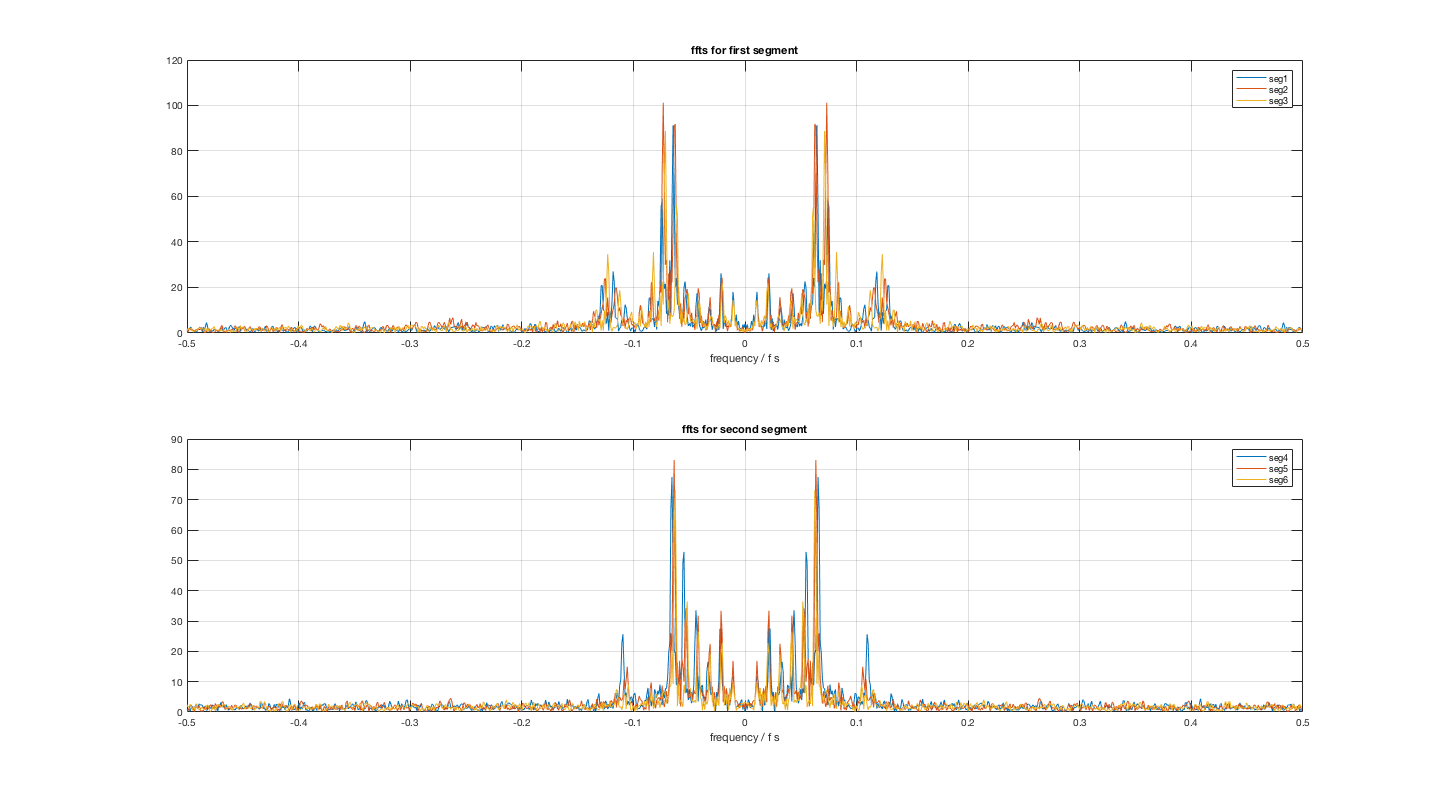
\includegraphics[scale=.25]{part_5_ffts_unvoiced.png}
  \caption{Comparing FFTs of Unvoiced Segments with Noise}
\end{figure}

\begin{figure}[H]
  \centering
  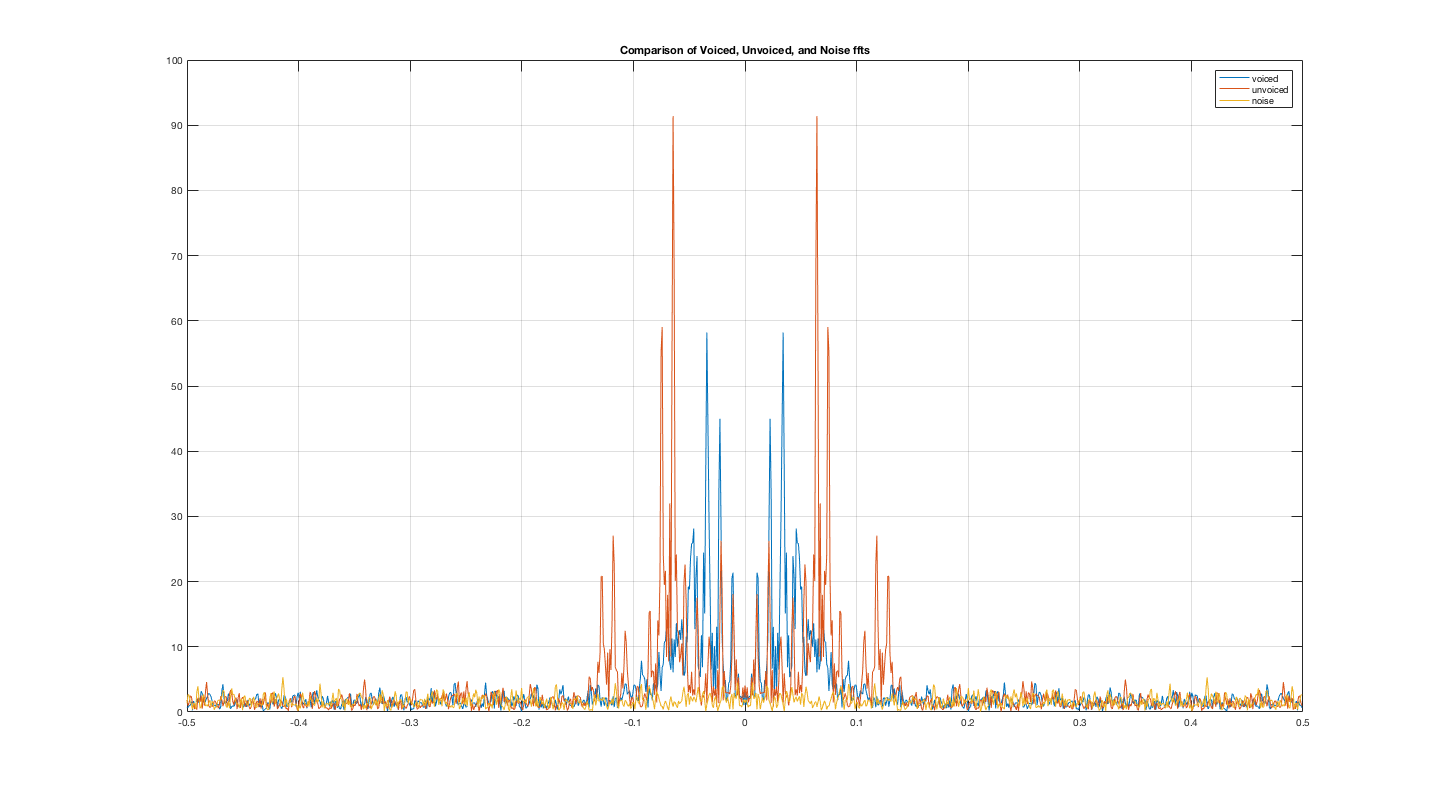
\includegraphics[scale=.25]{part_5_ffts_comparison.png}
  \caption{Comparing FFTs of Voiced, Unvoiced, and Silenced Segments with Noise}
\end{figure}

In terms of identifying voiced, unvoiced, and silenced segments based on the frequency domain, we came up with several different ideas, implemented two of them, and had mild success with one of them. Our thought process starting with wanting to use the known segments' frequency spectrum to identify voiced and unvoiced speech in our noisy recordings. In order to do so, we had to come up with some way of comparing the 'peaks' in each fft, or more precisely, comparing with frequencies were present in our known segments vs our unknown segments. The first idea was to simply find the frequencies with the highest coefficients and compare them straightaway. Basically the method sorts both ffts by coefficients, then compares the indexes of the highest valued frequencies in the results, if there is enough overlap, the ffts are the 'same'. 
\begin{lstlisting}
function match = compare_fft_hi_freqs(f1, f2, num, lim)
% Finds the highest num valued indexes between the arrays f1, f2. If more
% than lim of them match then the ffts are 'equivalent'

    [val1, index1] = sort(f1, 'descend');
    [val2, index2] = sort(f2, 'descend');

    index1=index1(1:num);
    index2=index2(1:num);

    s = intersect(index1, index2);

    match = length(s) >= lim;
end
\end{lstlisting}
This method, unfortunately, did not produce good results for separating voiced vs unvoiced speech. From reading documentation available on the Matlab website, as well as other forums, we learned that it was standard practice to use covariance or correlation matrices to compare signals. With that in mind, we implement another function that used the builtin Matlab method $corrcoef$ to get the correlation matrices of two FFTs and compare them that way:
\begin{lstlisting}
function match = correlate_fft(f1, f2)
% Uses correlation function to diff two ffts
    cor = corrcoef(f1, f2);
    match = cor(1,2);
end
\end{lstlisting}
While this method did produce some interesting results, it was not quite as accurate as we would have hoped. What is particularly interesting, however, is that the function was able to identify voiced speech in background noise in our original recording! Note the 'voiced' sections that were previously marked as silent.
Ultimately, we think that a combination of time and frequency domain analytics would be superior in determining voiced vs unvoiced speech, but did not include it as part of this report.

\begin{figure}[H]
  \centering
  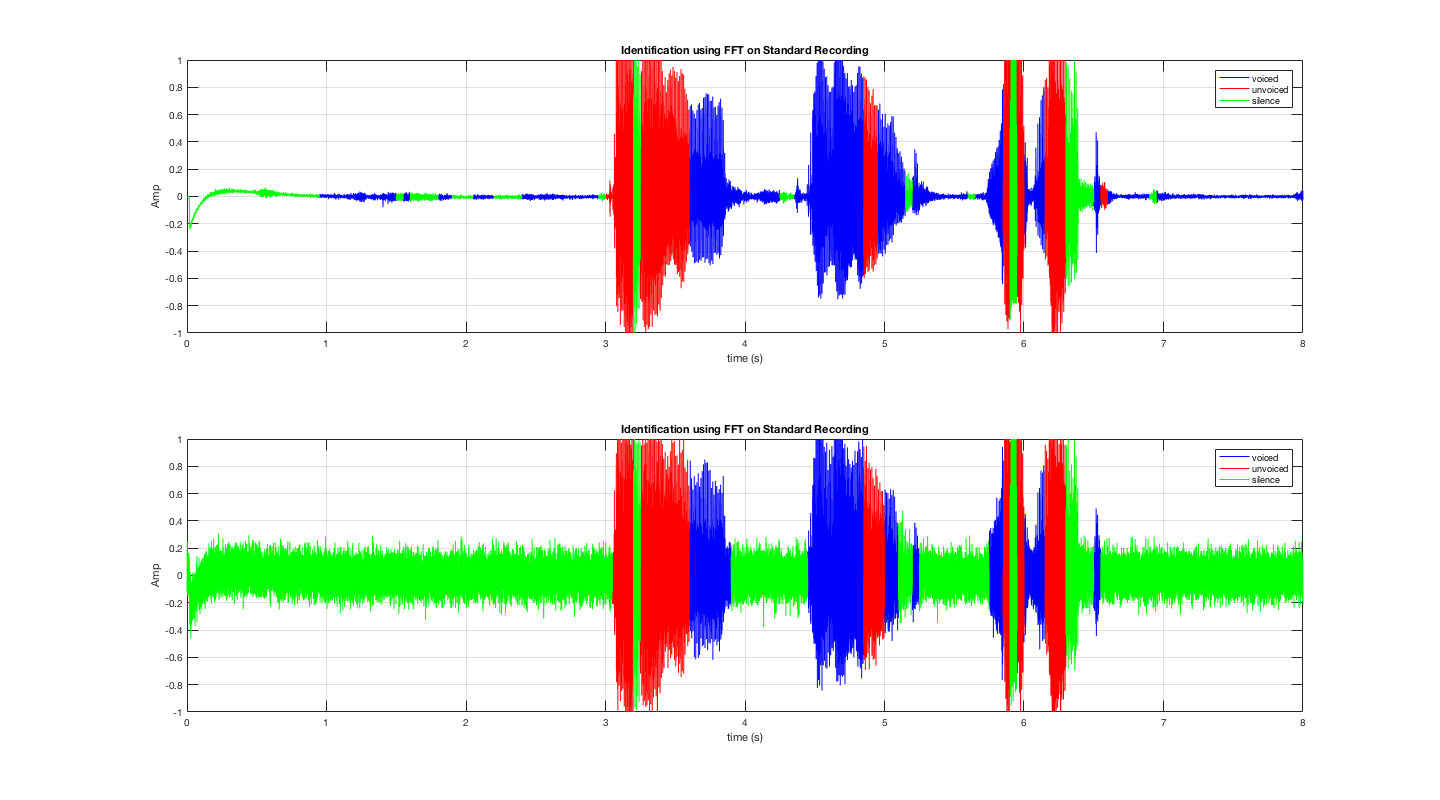
\includegraphics[scale=.25]{part_7_attempt.png}
  \caption{Labeling Voiced, Unvoiced, and Silence Segments for Regular and Noisy Signals with the FFT.}
\end{figure}


\subsection{Parts 8, 9}
We began by messing around on the command line, just seeing what different implementations of built-in-Matlab filters did. Ultimately we chose, in addition to the moving average filter, a few other filters to try out. In particular, since we knew the approximate frequency ranges for voiced and unvoiced speech from parts 5 and 6, we thought it might be useful to also try out a low pass and a pass band filter centered around those known values. As shown in figure 8, each filter was able to remove quite a bit of noise, but we also noted that each filter deformed the original recording in some odd way. For example, the moving average filter, while removing quite a bit of the white noise, also drastically 'evened' out the speech portion of our recording. Note the amplitude drops in the figure. Increasing the window size had the effect of further reducing white noise, but also almost dropping out our actual recording.
\begin{figure}[H]
  \centering
  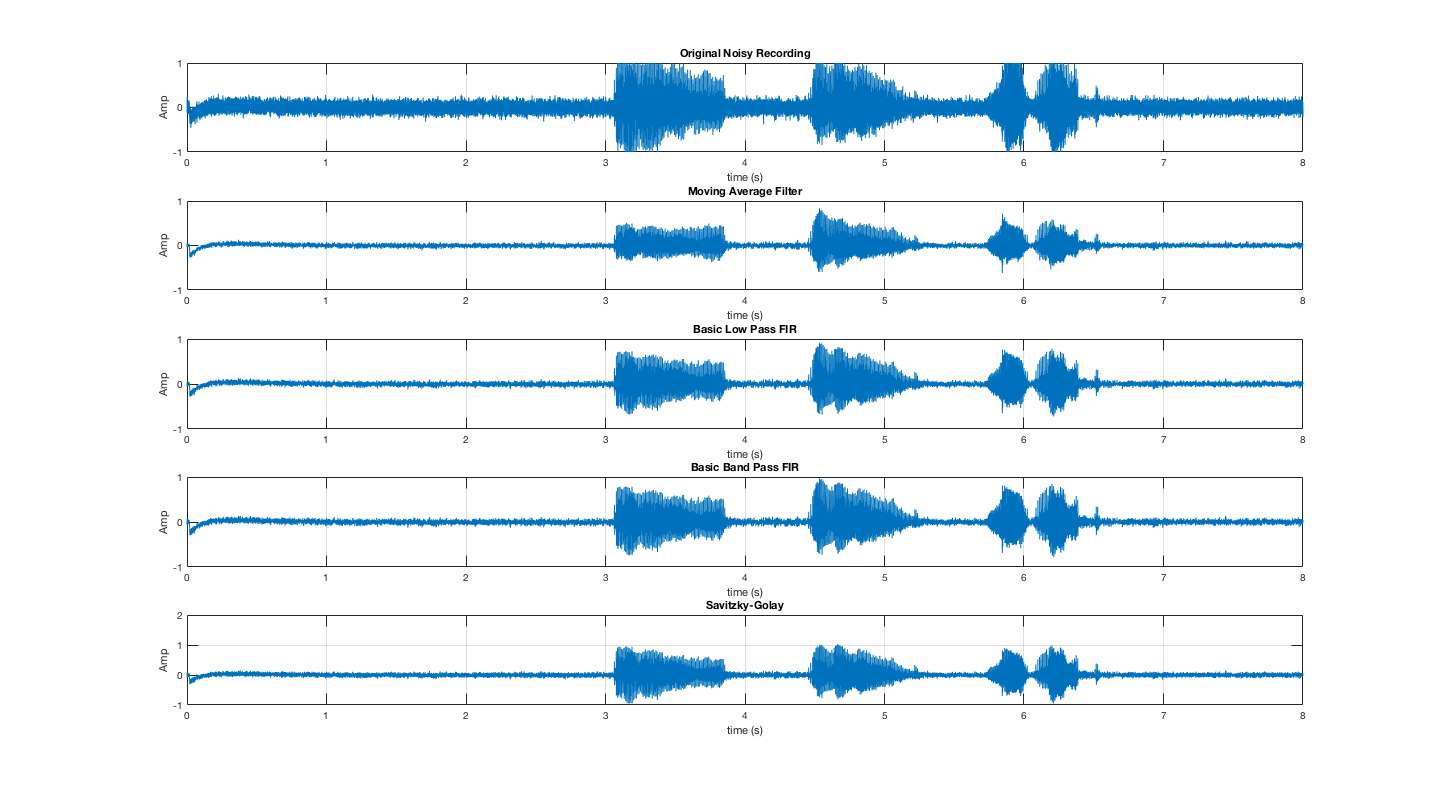
\includegraphics[scale=.25]{part_8_filter_visuals.png}
  \caption{Plotting Results of Different Filters on the Noisy Signal}
\end{figure}

Recalling from part 4 how our previously defined levels for $E_s$, $Z_s$, and $S_s$ were rendered completely useless by the addition of noise, we repeated, with mixed results, the process on our filtered signals. By bumping $S_s$ up slightly, we were able to correctly identify noise in all cases, but the filters also increased the zero-crossing rate in voiced speech, leading to other incorrect identifications in our results.
\begin{figure}[H]
  \centering
  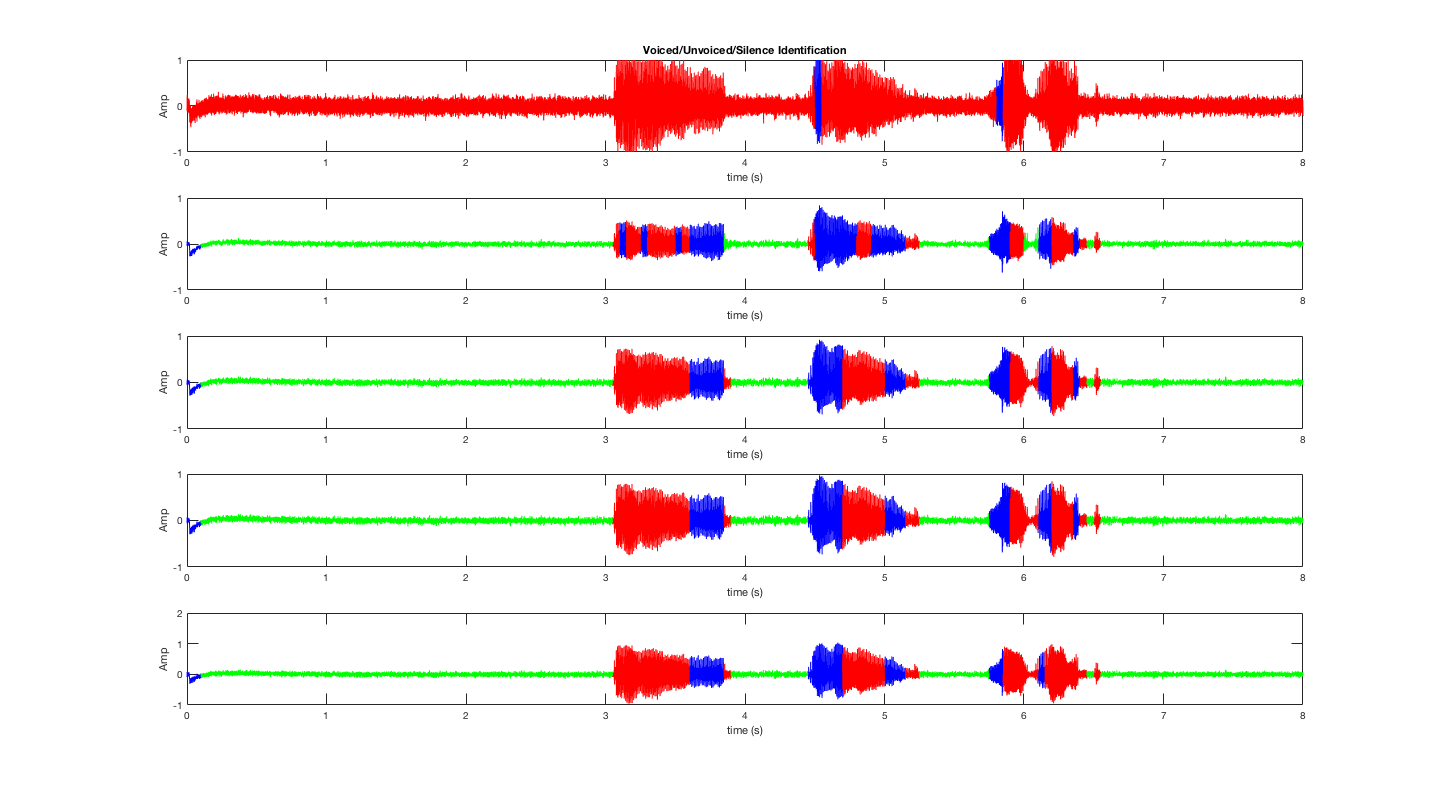
\includegraphics[scale=.25]{part_9_labeling_comparison.png}
  \caption{Filtered Signal Voiced/Unvoiced/Silence Identification}
\end{figure}

%
%
% Conclusion section
%
%
%
\section{Conclusion}
In terms of overall discovery, we would say that one major conclusion from this lab is that there is no notion of a 'one size fits all' approach for any portion of this lab - voiced/unvoiced labeling, Fourier spectrum comparison, and filtering all seem to require specific approaches for individual cases.

In part 3, we were able to get pretty close to automatically labeling voiced and unvoiced segments in our recording. Note however, that we had to write separate scripts in order to tune each level to the specific recording. We also found that different voices and different microphones would require different values for $E_s$, $Z_s$, and $S_s$. For example, recording using a headset vs recording using a laptops built in mic. The headset had very little background noise, but really bumped up the amplitude in our speech, where as the built in mic on the laptop did the opposite.

In part 7, we worked with a few different methods to extract voiced and unvoiced speech using the frequency spectrum, and only had mild success. From reading additional papers and online discussion boards, it was clear that there are an incredible amount of methods for comparing frequency spectrums. Many of them seem to be built into Matlab as well, and it would be interesting in the future to try out more of these more accepted methods. For this lab however, we mostly just brainstormed our own ideas of how to compare the FFTs.

In parts 8 and 9, we found that each filter performed well in a different way. The filters that were particularly good at filtering out white noise also seemed to have the effect of reducing the quality of the speech. Whereas those that maintained the quality of speech had a lot of residual white noise left in the recording. That being said, the fact that Matlab as a huge amount of built in filters with highly configurable options makes it very easy to try a large amount of different approaches and just see what works best. 


%
%
% Code section
%
%
%
\section{Code}

\begin{itemize}

\item Part-3 function for picking and returning voiced, unvoiced, and silenced portions of an audio sample.

\begin{lstlisting}
function [voiced, unvoiced, silence, t] = part_3(speech, fs, ...
    zc_threshold, en_threshold, silence_en_threshold, f_size)
% This computes voiced, unvoiced, and silence arrays passed in through the
% Specified limits
    %{
    Following:
    https://www.asee.org/documents/zones/zone1/2008/student/ASEE12008_0044_paper.pdf
    %}

    x = 1:length(speech);
    t = x./fs;

    len = length(speech);
    num_F = floor(len/(f_size));
    beg = 1;
    en = f_size;

    for i = 1:num_F
        speech_frame = speech(beg:en);

        % Compute zero crossings and energy for the frame
        zc = zero_crossings(speech_frame);
        theta = sum(abs(speech_frame))/length(speech_frame);
        energy(beg:en) = theta;
        crossing(beg:en) = zc;

        % Check for zc threshold
        ts = zc/f_size <= zc_threshold;
        es = theta >= en_threshold;
        voiced_i(beg:en) = (ts && es);

        % 'Silence' is low energy
        silence_i(beg:en) = theta < silence_en_threshold;

        % Check for energy threshold
        beg = beg + f_size;
        en = en + f_size;
    end

    [voiced, unvoiced] = split_vectors(speech, voiced_i); 
    [silence, unvoiced] = split_vectors(unvoiced, silence_i);

end
\end{lstlisting}


\item Zero-crossing Function used in part 3.
\begin{lstlisting}
function num_crossings = zero_crossings(xx)
% Count and return the number of 0 crossings in the vector, xx.

num_crossings = 0;
for i = 1:length(xx) - 1
    num_crossings = num_crossings + abs(.5 * sign(xx(i)) - .5 * sign(xx(i+1)));
end
\end{lstlisting}

\item Function for splitting up a vector into two vectors based on boolean indexes.
\begin{lstlisting}
function [xx, yy] = split_vectors(values, indexes)
% split_vectors separates values into 2 vectors of length values.
% xx[i] == values[i] when index[i] == 1, 0 o/w
% yy[y] == values[i] when index[i] == 0, 0 o/w
xx = values;
yy = values;

for i=1:length(indexes)
    if indexes(i)
        yy(i) = NaN;
    else
        xx(i) = NaN;
    end
end
end
\end{lstlisting}


\item Part\_7.m, used for identifying voiced, unvoiced, and silenced portions of speech.
\begin{lstlisting}
function [voiced, unvoiced, silence, t] = part_7(speech, fs, N, f_size,...
   voiced_model, unvoiced_model, lim)
% Determines voiced, unvoiced, and silenced segments using the fft using
% predetermined frames within a signal.
% speech - recorded data
% fs - sample rate
% N - fft order
% f_size - frame size
% voiced_model - known fft of voiced speech
% unvoiced_model - known fft of unvoiced speech
    
    % Compute ffts for voiced and unvoiced models
    voiced_fft = abs(fft(voiced_model,N));
    voiced_fft = fftshift(voiced_fft);
    unvoiced_fft = abs(fft(unvoiced_model,N));
    unvoiced_fft = fftshift(unvoiced_fft);
    
    x = 1:length(speech);
    t = x./fs;

    len = length(speech);
    num_F = floor(len/(f_size));
    beg = 1;
    en = f_size;

    for i = 1:num_F
        speech_frame = speech(beg:en);

        % Compute fft for the frame
        X = abs(fft(speech_frame,N));
        X = fftshift(X);
        
        % Does this match unvoiced fft?
        if correlate_fft(X, voiced_fft) >= lim
            voiced_i(beg:en) = 1;
            unvoiced_i(beg:en) = 0;
            silence_i(beg:en) = 0;
        elseif correlate_fft(X, unvoiced_fft) >= lim
            voiced_i(beg:en) = 0;
            unvoiced_i(beg:en) = 1;
            silence_i(beg:en) = 0;
        else
            voiced_i(beg:en) = 0;
            unvoiced_i(beg:en) = 0;
            silence_i(beg:en) = 1;
        end

        % Increment
        beg = beg + f_size;
        en = en + f_size;
    end

    [voiced, v] = split_vectors(speech, voiced_i); 
    [unvoiced, v] = split_vectors(speech, unvoiced_i); 
    [silence, v] = split_vectors(speech, silence_i);
end
\end{lstlisting}


\end{itemize}


\end{document}